\documentclass[a4paper,12pt,hidelinks]{report}

%%Pacchetti utili anche se non necessari

\usepackage{amsfonts}
\usepackage{amsmath}
\usepackage{latexsym}
\usepackage{tabularx}
\usepackage[italian]{babel}
\usepackage[bookmarks=true]{hyperref}
\usepackage{url}
% \usepackage{subfigure}
\usepackage{epstopdf}
\usepackage[utf8]{inputenc}
% \usepackage[utf8x]{inputenc}
\usepackage{listings}
\usepackage{graphicx}
%-------------------------------------------

% \title{Progettazione sito web\\ ''B\&B La Vecchia Posta''}
% \author{Daniele Di Pompeo \\mat. 226766}
% \annoaccademico{2013-2014}
\begin{document}
  \begin{titlepage}
    \begin{center}
    % Upper part of the page
      
\includegraphics[width=0.5\textwidth,keepaspectratio=true]{../img/logo}\\[1cm]    
      \textsc{\LARGE Mappa del sito}\\[0.6cm]
      \textsc{\LARGE  progetto:\\[0.5cm] ``B\&B La Vecchia Posta''}\\ [2.0cm]

    % Author and supervisor
      \begin{minipage}{0.8\textwidth}
	\begin{flushleft} \large
	  \emph{Autore:} Daniele Di Pompeo \\[0.5cm]
	  \emph{Versione documento: 1.0}\\[0.5cm]
	  \emph{Data emissione del documento: \today}\\[0.5cm]
	\end{flushleft}
      \end{minipage}
    \end{center}
  \end{titlepage}

La figura fig.\ref{fig:sitemap} mostra graficamente la struttura gerarchica del sito. 
\begin{figure}[h!]%
    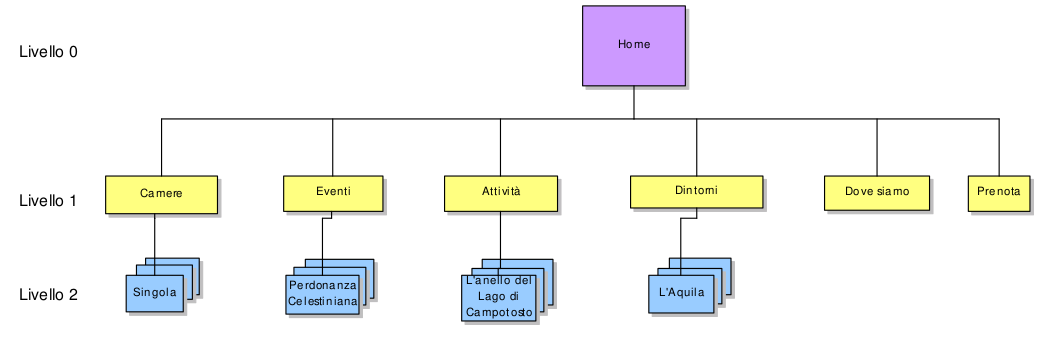
\includegraphics[width=1\textwidth,keepaspectratio=true]{../img/sitemap}
    \centering
    \caption{Mappa del sito}%
    \label{fig:sitemap}%
\end{figure}

La figura \ref{fig:navigazione} mostra la totalità dei percorsi del sito, successivamente verranno analizzati nel dettaglio per le singole sezioni del sito.
Per avere una maggiore leggibilità dello schema si è scelto di utilizzare la notazione abbreviata.
\par Si è scelto di inserire la pagina \textit{prenotazione}, che nella scaletta dei contenuti \footnote{Vedere documento dei requisiti punto 2.1.1} non è presente.
\par Nei diagrammi realizzati con il CASE è stato utilizzato il seguente schema di colori per semplificare la lettura:
\begin{itemize}
 \item \textbf{Nero}: collegamenti verticali
 \item \textbf{Giallo}: collegamenti orizzontali
 \item \textbf{Verde}: collegamenti trasversali
 \item \textbf{Rosso tratteggiato}: scorciatoia
\end{itemize}

\begin{figure}[h!]%
    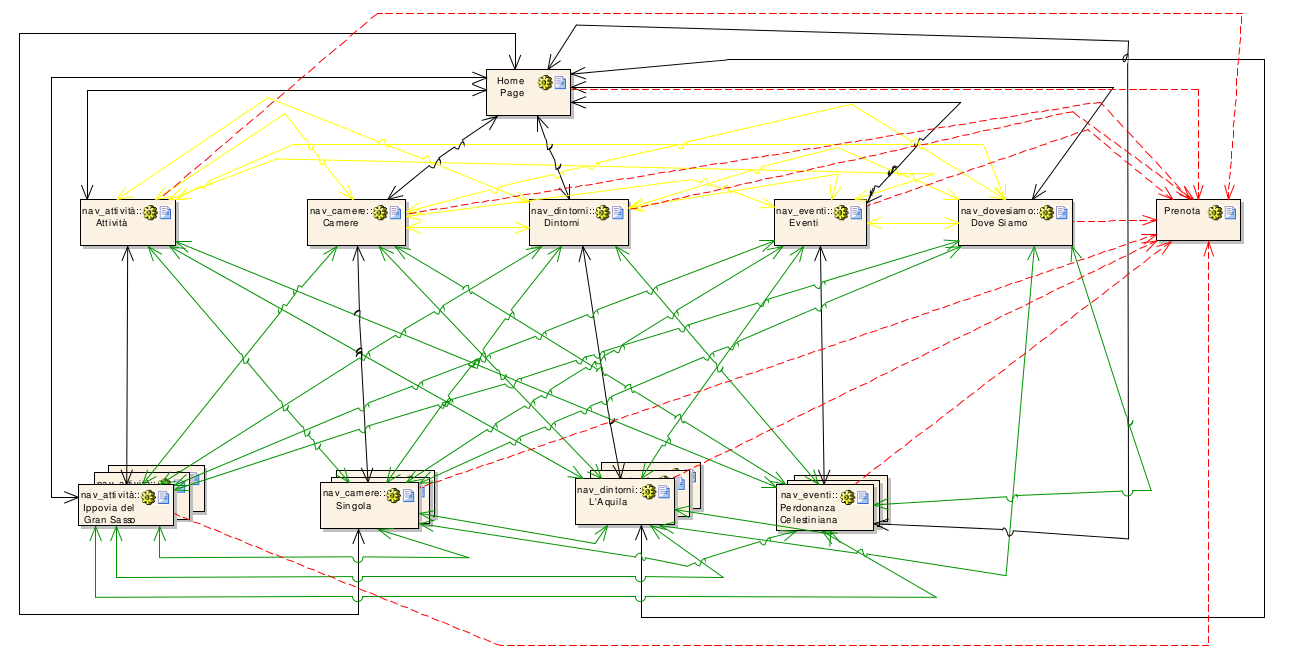
\includegraphics[width=1.2\textwidth,keepaspectratio=true]{../img/navigazione}
    \centering
    \caption{Possibili percorsi all'interno del sito}%
    \label{fig:navigazione}%
\end{figure}

\newpage
\paragraph{Sezione: Camere}

La figura \ref{fig:nav_camere} mostra i possibili percorsi percorribili dalla sezione camere e sue sotto-sezioni.

\begin{figure}[h!]%
    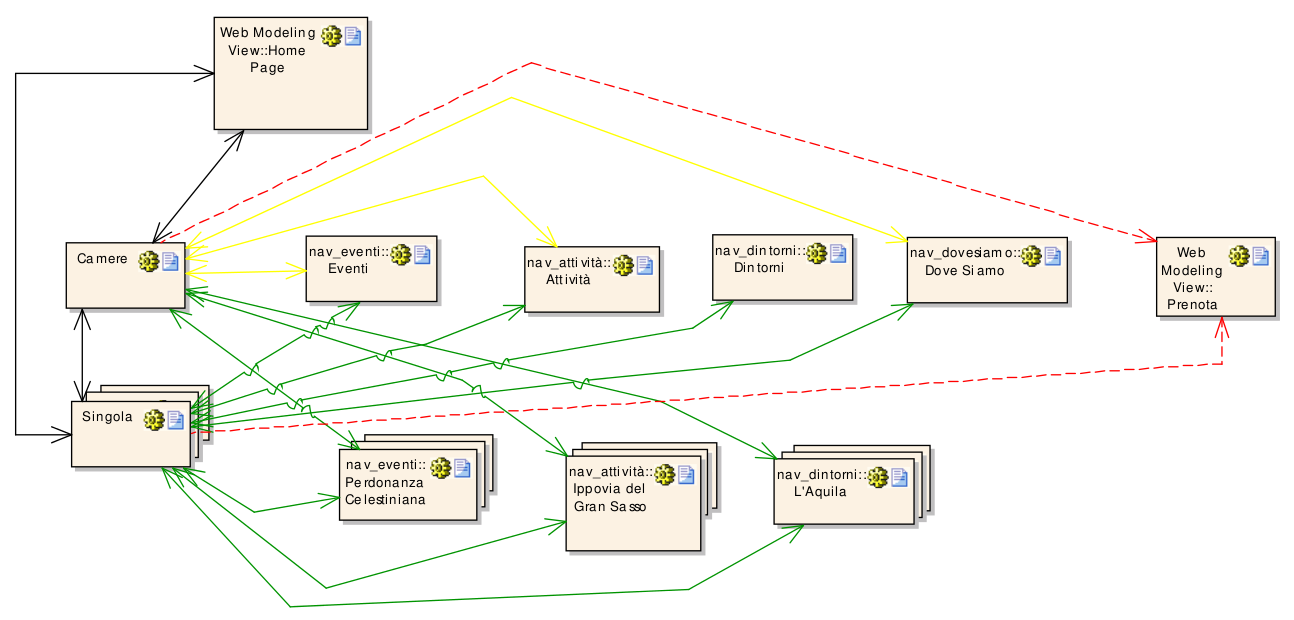
\includegraphics[width=1.1\textwidth,keepaspectratio=true]{../img/nav_camere}
    \centering
    \caption{Possibili percorsi della sezione camere}%
    \label{fig:nav_camere}%
\end{figure}

\newpage
\paragraph{Sezione: Attività}
La figura \ref{fig:nav_attivita} mostra i possibili percorsi che si possono eseguire dalla sezione del sito \textit{attività} e sue sotto pagine.

\begin{figure}[h!]%
    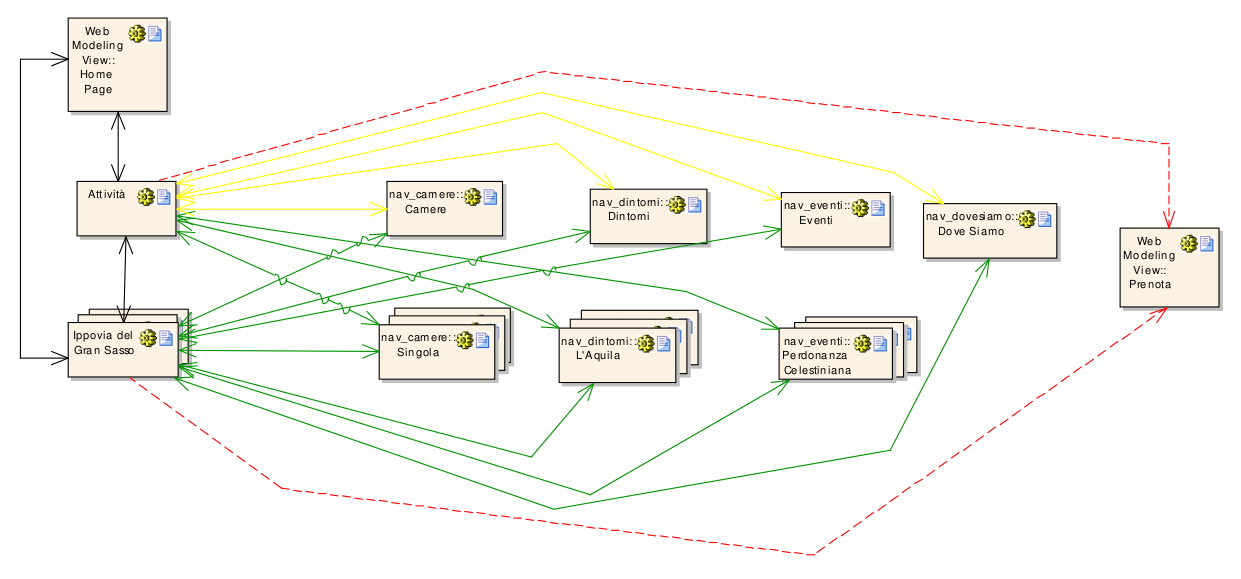
\includegraphics[width=1.1\textwidth,keepaspectratio=true]{../img/nav_attivita}
    \centering
    \caption{Possibili percorsi della sezione attivita}%
    \label{fig:nav_attivita}%
\end{figure}

\newpage
\paragraph{Sezione: Dintorni}
In questa sezione del documento vengono mostrati, in figura \ref{fig:nav_dintorni}, i tragitti che consentono all'utente di spostarsi da una sezione ad un'altra con il focus 
sulla sezione del sito \textit{ditorni} con le sue sotto pagine.

\begin{figure}[h!]%
    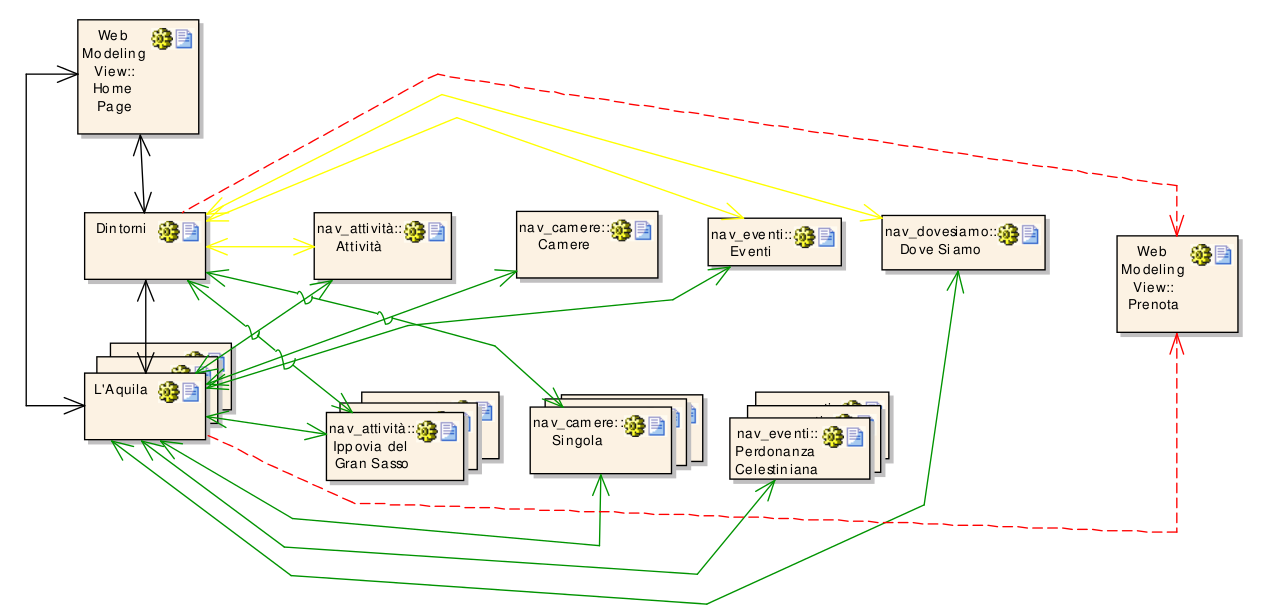
\includegraphics[width=1.1\textwidth,keepaspectratio=true]{../img/nav_dintorni}
    \centering
    \caption{Possibili percorsi della sezione ditorni}%
    \label{fig:nav_dintorni}%
\end{figure}

\newpage
\paragraph{Sezione: Eventi}
Si descrive con l'immagine \ref{fig:nav_eventi} i possibili tragitti partendo dalla sezione del sito \textit{eventi} e/o dalle sue sotto sezioni.

\begin{figure}[h!]%
    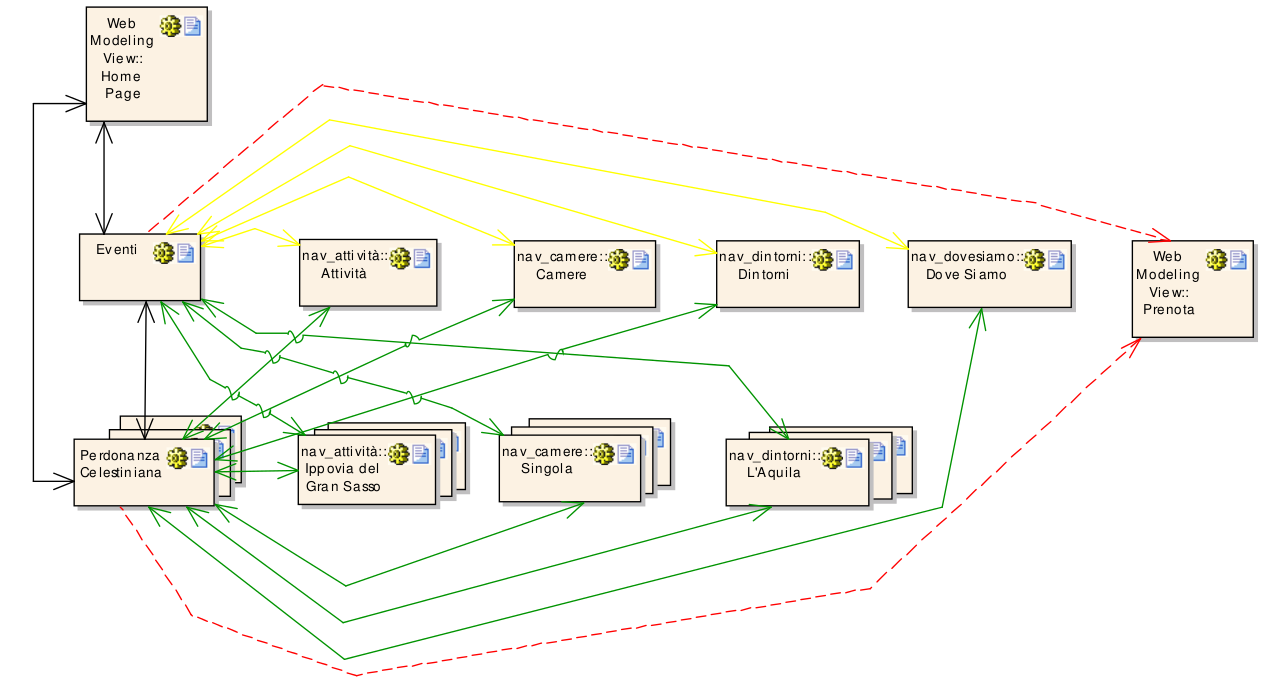
\includegraphics[width=1.1\textwidth,keepaspectratio=true]{../img/nav_eventi}
    \centering
    \caption{Possibili percorsi della sezione eventi}%
    \label{fig:nav_eventi}%
\end{figure}

\newpage
\paragraph{Sezione: Dove Siamo}
Si descrive con l'immagine \ref{fig:nav_dovesiamo} i possibili tragitti partendo dalla sezione del sito \textit{Dove Siamo}.

\begin{figure}[h!]%
    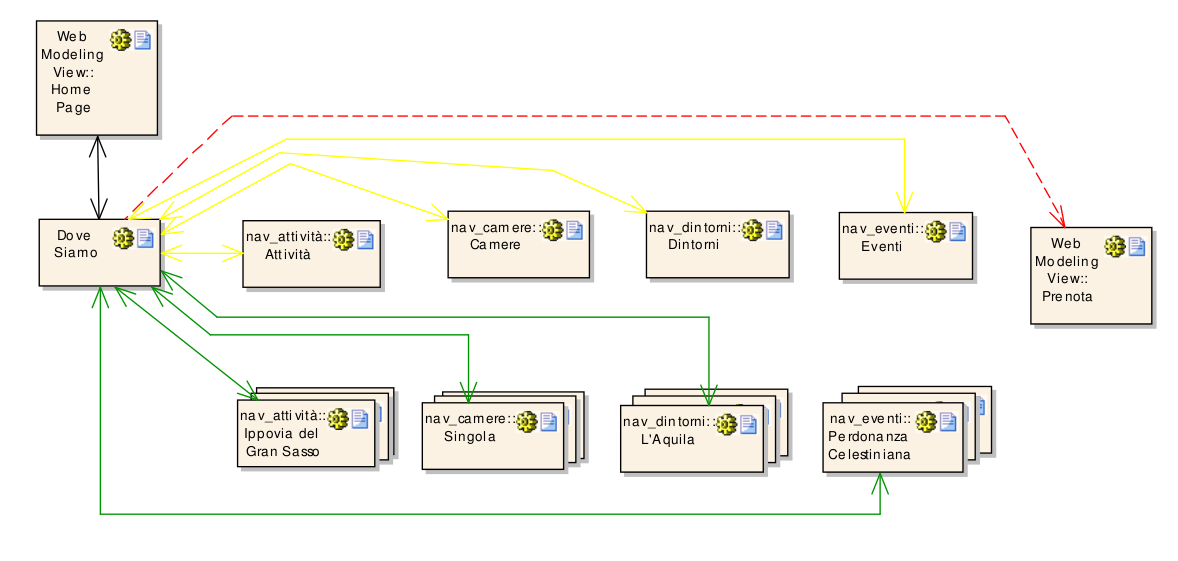
\includegraphics[width=1.1\textwidth,keepaspectratio=true]{../img/nav_dovesiamo}
    \centering
    \caption{Possibili percorsi della sezione eventi}%
    \label{fig:nav_dovesiamo}%
\end{figure}

\paragraph{Alcune osservazioni finali}
Si nota come la scelta di inserire una scorciatoia alla pagina \textit{prenotazione} abbia reso la pagina sempre accessibile facilmente da qualsiasi sezione 
interna del sito. Questa scelta di progettazione si auspica porti ad un aumento delle richieste di prenotazione.
\end{document}          
